\documentclass{standalone}
\usepackage[utf8]{inputenc}
\usepackage[svgnames]{xcolor}
\usepackage{tikz}
\usetikzlibrary{fit,shapes,positioning}


\begin{document}
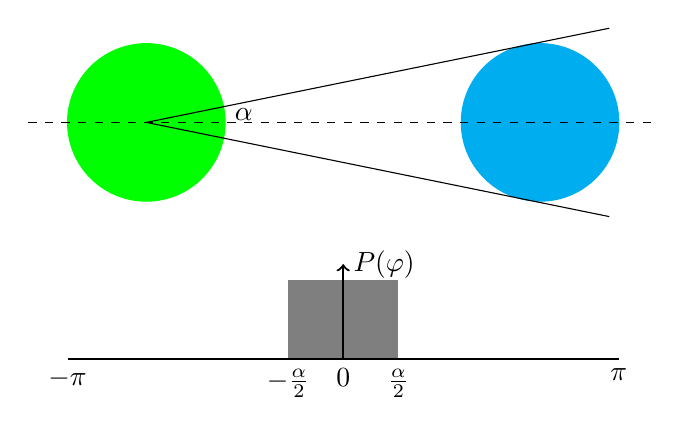
\begin{tikzpicture}[
        graph/.style={fill=black, draw opacity=0, fill opacity=0.5}
    ]
    
    \filldraw[green] (0,0) circle (1cm) coordinate (a) ;
    \filldraw[cyan] ([xshift=5cm]a) circle (1cm) coordinate (b) ;
    \draw (a) -- (11.5:6cm) ;
    \draw (a) -- (-11.5:6cm) ;
    \node[right=1cm of a, yshift=0.1cm] {$\alpha$} ;

    \draw[dashed] ([xshift=-1.5cm]a) -- ([xshift=1.5cm]a -| b) ;

    \coordinate (x0) at ([xshift=-1cm, yshift=-3cm]a) ;
    \coordinate (x1) at ([xshift=1cm]x0 -| b) ;

    \draw[thick] (x0) to
        node[pos=0,below]{$-\pi$}
        node[pos=0.4,below]{$-\frac{\alpha}{2}$} coordinate[pos=0.4] (alpha0)
        node[pos=0.5,below]{$0$} coordinate[pos=0.5] (y0)
        node[pos=0.6,below]{$\frac{\alpha}{2}$} coordinate[pos=0.6] (alpha1)
        node[pos=1,below]{$\pi$} (x1);

    \draw[thick, ->] (y0) -- ([yshift=1.2cm]y0) node[right]{$P(\varphi)$} ;
    \draw[graph] (alpha0) rectangle ([yshift=1cm]alpha1)  ;
    
\end{tikzpicture}
\end{document}